\documentclass[12pt]{IEEEtran}

\usepackage{cite}
\usepackage{hyperref}
\usepackage{graphicx}

\begin{document}

\title{Artificial Neural Network Classifications: Predicting NFL Game Outcomes}

\author{Jason Melnik}
\maketitle

\begin{abstract}
	Artificial Neural Network's(ANN's) have been used to predict sports using classification for the past two decades with increasing accuracy. Each attempt has had different methodologies and technologies to try and achieve higher results than the previous. Gambling has been a high driving factor for most people when it comes to NFL games and having a higher chance of winning can be beneficial. Historical ANN's have used models that have the features of historical matches, opposition information, player performance, and betting odds. In this article the features of the ANN's will be the individual players statistics. This article aims to acheive higher accuracy than previous attempts by including more features. This article will hopefully help others in finding a better ANN's to predict the results of a NFL game.
\end{abstract}

\section{Introduction}
	Machine Leaning(ML) is using unseen data to predict a target variable through classification. Classification models need training data and validation data sets to train the model in finding the best weights for predicting the target variable. This article will be building a classification model to predict one class variable either win or lose. The trained model will then try and predict the results of the 2020 NFL season. The model will be built using many techniques that are similar to past authors that have made classification ANN.

\section{History}

One of the initial studies of predicting sport results was Purucker\cite{NNQ}. They used an ANN model with the features of yards gained, rushing yards gained, time of possession, betting line odds, and turnover margin. Backward-propagation paired with the ANN helped Purucker achieved 61\% accuracy while the domain experts achieved 72\% accuracy. Purucker had limitations such as a small amount of features was used. They concluded that using the back-propagation algorithm was the most effective approach. Then came Kahn\cite{kahn2003neural} which extended the researchh of Purucker and concluded their research with a higher accuracy. Khan's prediction model performed better than experts in the NFL. The data used was 208 matches from 2003 and the features was rushing yard differential, total yardage differential, turnover differential, home team indicator, and away team indicator. The winner was classified as 1 while the loser would be classified as -1 to try and solve this using classification. Khan used a network of 10-3-2 with an accuracy of 75\% while domain experts were 63\% accurate. 

Then came McCabe and Trevathan\cite{mccabe2008artificial} attempting to predict results in AFL, NFL, Super Rugby, and EPL. The data they used included all past games back to the year 2002. They used a multi-layer perceptron which was an old version of ANN's with back-propagation, and conjugation-gradient algorithms. Their neural network was 20-10-1. Their ANN performance was 67.5\% accurate compared to domain experts 60\% accuracy. 

Tax and Joustra\cite{tax2015predicting} built several different classification models for Dutch football. Their data consisted of 13 years of past games and 1 to 51 features of every game. They wanted to see how a model with betting odds would compare with a hybrid model of betting odds and match features. They were also one of the first to mention that cross validation is not appropriate for when predicting sports since the time ordered nature of the data. There was nine classification algorithms used when conducting this experiment which included Bayes, NN with BP, LogitBoost, CHIRP, Random Forest, FURIA, C4.5, hyper pipes, and DTNB. When using only betting odds the highest accuracy was 55.5\% with the FURIA classifier. The public data models that achieved the highest accuracy was ANN and Bayes with an accuracy of 54.7\%. The hybrid model of the LogitBoost with Relief attribute selection achieved the highest accuracy of 56.1\%. They also concluded that the difference between the betting odds model and public data model were not statistically significant according to McNemar's test. This shows that using betting odds alone is a reasonable predictor for predicting a sports outcome.  

\section{Neural Networks}
When predicting outcomes of sports most use classification with the class of win, loss, or draw to predict while others use numeric predictions where they predict winning margins\cite{bunker2019machine}. Most previous studies have applied Artificial Neural Networks(ANN) to predict sport results but they have all used general data. The previous studies have used team data or betting data but this paper will use player statistics instead. "An ANN usually contains interconnected components (neurons) that transform a set of inputs into a desired output"\cite{bunker2019machine}. ANN works from using non-linearity of hidden neurons with adjusting weights that contribute to the final decision. ANN will have an output that relies on components associated with the network and importantly the input features. A trained ANN model is constructed after a training data set is used as input for the ANN to adjust its weights to fit a pattern that it finds. The changes to weights in the ANN algorithm is to try and fulfill the desired model's accuracy that is assigned by the user. In our case is how accurate it can predict if a team will win or lose. The ANN takes in the input and tries to classify if it's a win or loss, but if it fails on classifying it then it will use the back propagation algorithm. The back propagation algorithm adjusts the weights for the next input hoping that the new adjusted weight will be a better pattern in finding the correct classification. 

\section{Data}

To get the necessary data for this project we need to scrape the website  \href{https://www.pro-football-reference.com/}{Pro Football Reference} which provides us with statistics of every player and game. The data scraped will include past games and their starting roster. The data will be from footballs games in the year 2010 to 2020. Once all the roster data is scrapped the individual player statistics are next. The offense players data include defense interceptions, fumbles, tackles, rushing, receiving, and some default statistics. The defense positions data include interceptions, fumbles, tackles, and defaults. The individual player data is then averaged by their entire career up until the given game. Offense and defense field positions will be represented as an integer since there are 51 different positions as strings. Each position will have a different length of features since positions have different statistics. Defense players have the same statistics no matter the position. Once we have every player statistic on the entire roster we combine all the individual player data into one list that represents a team. To represent one game it will be a combination of all the starters. The layout will be an integer list with both teams data within it, with the total length being 1304 variables. I then made a boolean random function to chose either have the winning stats first or second and correspond the result to it. For the results list it will be a list of 0s and 1s with 0 representing the winning team in the front of the list and 1 as the winning team at the end of the list. The entire data set will be the years 2010 to 2019 for training/validation while 2021 games will be the test data. The training data is 80 percent of the data while 20 percent is for validation data. The test data will be the 2020 NFL season. To better understand the data layout use this Figure\ref{fig:datavisualization}. 

\begin{figure}
	\centering
	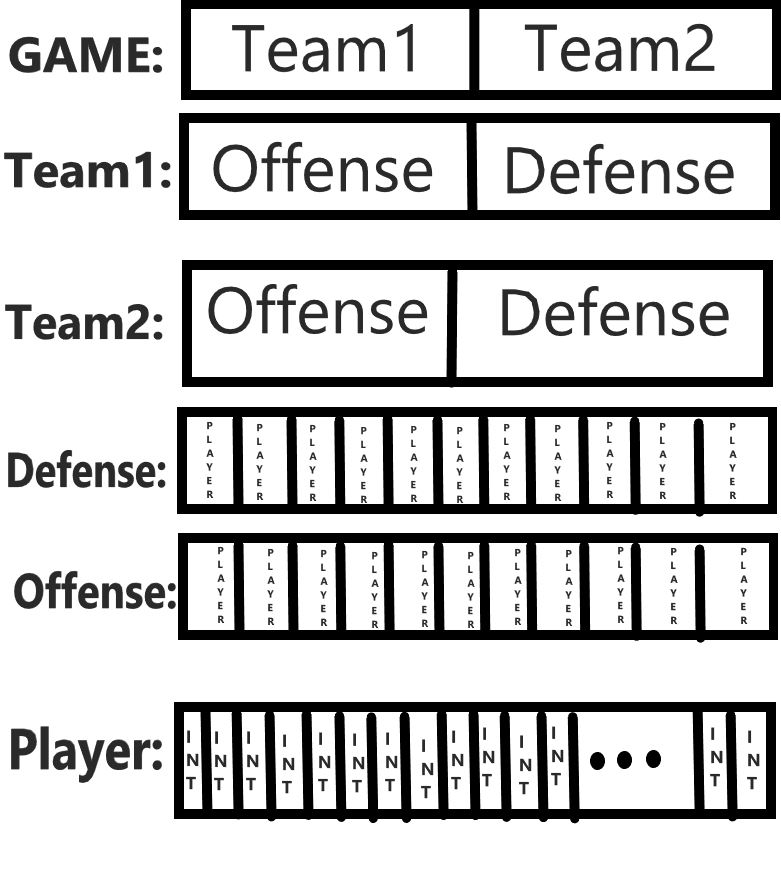
\includegraphics[width=1.0\linewidth]{../dataVisualization}
	\caption{}
	\label{fig:datavisualization}
\end{figure}

\section{Over Fitting Problem}
When training a model we run into the problem of over fitting which is when the training data doesn't generalize and instead tries to fit the training data. This can lead to failure when testing the network due to the model only finding patterns to the training data. To show this problem we demonstrate by using a tiny model that contains one dense layer of size 128. The accuracy of the model turns out to be 97 percent accurate but the validation data accuracy is only at 51 percent. This becomes a problem since we want to predict a game with high accuracy and having 51 percent is not enough. A good way to test if a model is over fitting is by tracking binary cross entropy loss on the test and validation data when trying a new model. It's normal for the loss function to have a small difference or if both metrics are moving in the same direction. Over fitting may be happening if validation loss begins to stagnate while the training loss improves. If the validation metric is going the wrong direction then the model is clearly over fitting. In Figure\ref{fig:tinymodel} the binary\_crossentropy validation and training have a huge difference. The solutions to this problem include adding weight regularization and Dropout layers. To limit over fitting there are easy methods to put constraints on the complexity of the network, this causes the weights to take in small values, which causes the distribution of weight values to become better regulated. We will be using "L2 regularizaion, where the cost added is proportional to the square of the value of the weights coefficients (i.e. to what is called the squared "L2 norm" of the weights). L2 regularization is also called weight decay in the context of neural networks"\cite{tensorflow2015-whitepaper}. So adding l2 regularizer with a rate of .000001 to the tiny model we get the results in Figure\ref{fig:regularizermodel}. This shows us that the loss in train and validation follow each others patterns closer, but the loss is still increasing. Another fix is adding a Dropout Layer with a rate of .9 on top of the regularizer to get a better fitted model. "Dropout, applied to a layer, consists of randomly "dropping out" (i.e. set to zero) a number of output features of the layer during training. Let's say a given layer would normally have returned a vector [0.2, 0.5, 1.3, 0.8, 1.1] for a given input sample during training; after applying dropout, this vector will have a few zero entries distributed at random, e.g. [0, 0.5, 1.3, 0, 1.1]"\cite{tensorflow2015-whitepaper}. We want to use dropout because individual nodes in the network cannot rely on the output of each other and each node needs output features that can be useful on their own. When adding a Dropout layer to our tiny model with the regularizer we get these results in Figure\ref{fig:regularizerdropoutmodel}. This shows a much better pattern where binary\_crossentropy is decreasing and following the same pattern. 

\begin{figure}[!]
	\centering
	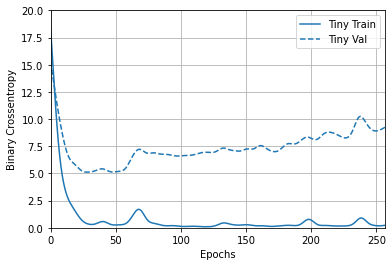
\includegraphics[width=0.7\linewidth]{Images/tinyModel}
	\caption{The binary\_crossentropy between training and validation data in a Tiny model that does not account for over fitting}
	\label{fig:tinymodel}
\end{figure}

\begin{figure}[!]
	\centering
	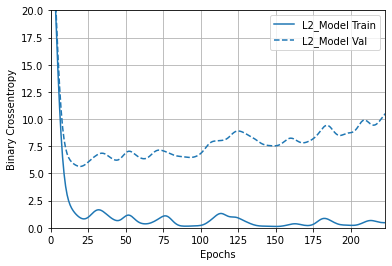
\includegraphics[width=0.7\linewidth]{Images/regularizerModel}
	\caption{The binary\_crossentropy between training and validation data in a Tiny model that adds a regularizer layer}
	\label{fig:regularizermodel}
\end{figure}

\begin{figure}[!]
	\centering
	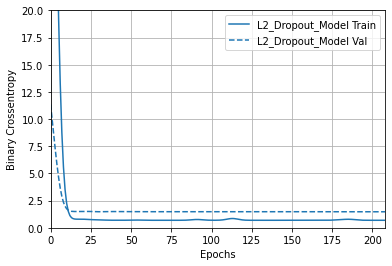
\includegraphics[width=0.7\linewidth]{Images/regularizerDropoutModel}
	\caption{The binary\_crossentropy between training and validation data in a Tiny model that adds a regularizer and dropout layer}
	\label{fig:regularizerdropoutmodel}
\end{figure}

\section{Tuning Hyper-parameters}
This section is to build the best model for our neural network with the highest validation accuracy. To quickly converge on a high-performing model I use the hyperband tuning algorithm which uses adaptive resource allocation and early stopping. This algorithm is done by using a sports championship style bracket. "The algorithm trains a large number of models for a few epochs and carries forward only the top-performing half of models to the next round. Hyperband determines the number of models to train in a bracket by computing 1 + logfactor(max\_epochs) and rounding it up to the nearest integer"\cite{tensorflow2015-whitepaper}. In the tuner has four Dense, Dropout, and regularized layers. The four Dense layers have a range of 2 to 1304 with increments of 1. The regularized rate ranges from 0.00001 to .1 with 0.00001 increments. Finally our Dropout layer has a rate that ranges from .01 to .50 with .01 increments. Keras tuner will go through hundreds of combinations to find the model that has the highest validation accuracy.

\section{Neural Network Binary Classification}
The neural network will have the input shape of 1304 to represent a game with two teams. There will then be two hidden layers with 64 neurons and one dropout layer between the hidden layers. The dropout layer has a .02 rate while the l2 regularizer has a 0.0008 rate. This Figure\ref{fig:diagram} shows a clear diagram of the ANN that will be trained and tested on. The output layer will be one neuron with Sigmoid activation. Sigmoid function transforms the values with the range of 0 and 1. The mathematical expression for sigmoid if f(x) = 1/(1+e\^-x). This is our output activation because we want to classify the output in either 0 or 1 and sigmoid does that well. If the output value less than .50 then it's 0 and if it's greater then it's classified as 1. The hidden layers have an Exponential Linear Unit(ELU) activation which modifies the slope of the negative part of the function of ReLU function. ELU uses a log curve for defining negative values with the function f(x) = x, x>= 0 | f(x) = a(e\^x-1), x<0. ELU is the best activation compared to others due to several tests performed and many others believe it to be great for classification problems. The model will have binary crossentropy loss function with accuracy metrics to determine if the model is improving with each epoch. When doing 0 or 1 classification its common to use binary crossentropy. This loss functions compares each of the predicted probabilities to the actual result output and calculates the score than penalizes the probabilities based on the distance from the expected value. That's why the closer it is to 0 the better the model is. Finally the accuracy metric is just a percentage of how correct the model is to predicting the actual result. With these technologies we can now train our model. 

\begin{figure}
	\centering
	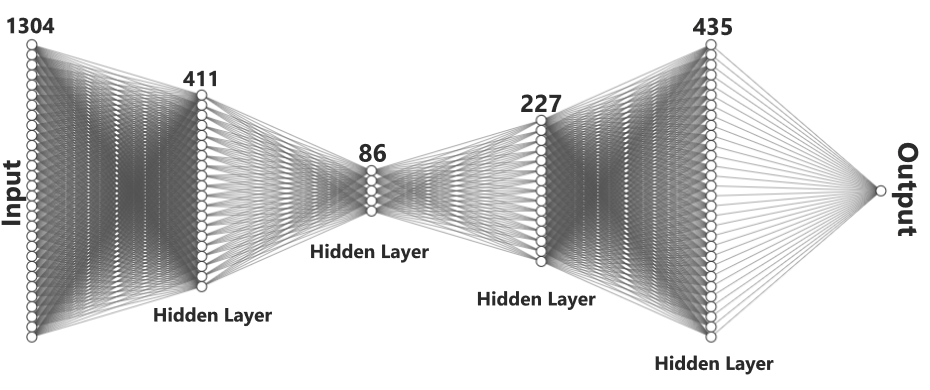
\includegraphics[width=0.7\linewidth]{../diagram}
	\caption{}
	\label{fig:diagram}
\end{figure}


\section{Results}
The model achieved 61\% accuracy on the training data. This resulted in 57\% accuracy for validation data. When training the ANN with the validation data the resulting binary crossentropy is shown in Figure\ref{fig:finalbinary}. This binary crossentropy shows that the loss in test and validation data was going down and in the same direction which is perfect for training ANN. This Figure\ref{fig:finalaccuracy} shows that the accuracy of both training and validation data go up as the epochs go up which is another sign that the ANN is getting trained perfectly. For the 2020 NFL games I ran the model 10 times to get an average of what the accuracy would be and ran it for 100 epochs to train the model. So for the 2020 NFL games the ANN has a 54.49\% accuracy, 61.51\% accuracy being the highest, and 47.87\% accuracy being the lowest when running the 10 trials. 

\begin{figure}
	\centering
	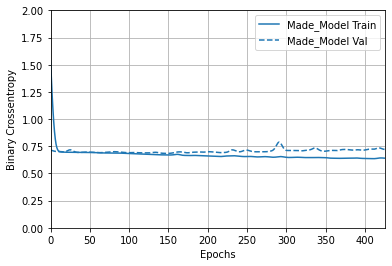
\includegraphics[width=0.7\linewidth]{../final_binary}
	\caption{}
	\label{fig:finalbinary}
\end{figure}

\begin{figure}
	\centering
	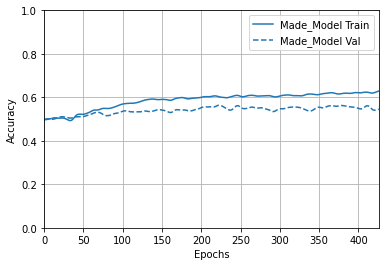
\includegraphics[width=0.7\linewidth]{../final_accuracy}
	\caption{}
	\label{fig:finalaccuracy}
\end{figure}

\section{Additional Comments}
If there was more time for this project I would try different activation functions, optimizers, loss functions, and data sets. For the data there may be to much data for each player and more data exploration may lesson the data points. Another options would be to average the team data and use that as input. Using an official API from NFL.com or ESPN.com would have been much easier for getting the data. As for data using only personal statistics like weight, speed, and more could provide better results. There are just so many other routs to take and there is a possibility of having much higher results than what was achieved in this article. The main goal of this article was just to see if it would be possible to determine winners using all the statistics of each player. 

\section{Conclusion}
With these results it is possible to use this ANN to predict future games with little profits since it's slightly above 50\%. This article shows that using player statistics is not the best method in finding the winner in an NFL match. ANN are evolving every day with new and better technologies coming out with a possibility that one day you could predict the winner of an NFL match. 

\newpage
\bibliographystyle{IEEEtran}
\bibliography{./references}

\end{document}